\section{Motivating Example} \label{sec:motivating_example}

 \begin{figure*}[t]
    \centering 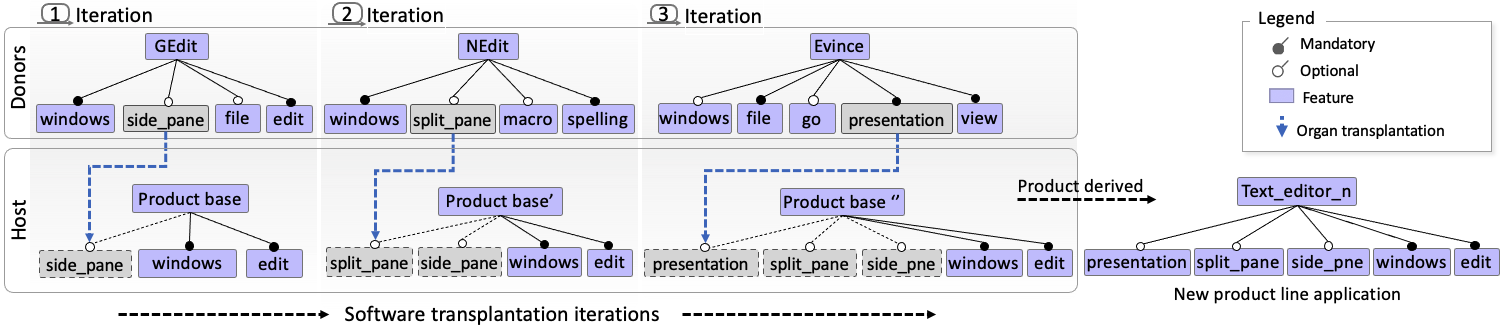
\includegraphics[width=\textwidth]{images/incremental_ST4.png}
    \caption{Product derivation process using the \FOUNDRY approach. \textit{\prodscalpel transplants three features, in sequence, into the GEdit's product base to derive a new text editor after three iterations of organ transplantation.} }
    \label{fig:incremental_pd}
\end{figure*} 
 %COMMENT: \ls{The case for SPL needs to be elaborated:  we must argue that the various GNOME subprojects share sufficient code to define a product base.  If too many of them are too different, SPL would be inappropriate.}
%\todo{This sentence is problematic:  we shoudl discuss. Done}
%\eb{from Leandro: I've rewritten this sentence by providing details of how GNOME could benefit from using SPLE principles as mass customisation and a common platform.}

\textbf{ORIGINAL VERSION}

The open-source GNOME project\footnote{https://wiki.gnome.org/Projects} encompasses a large portfolio of individual programs evolve as independently as possible from the rest. These programs share features, but because they are separately developed, their constituent features cannot be easily reused across its portfolio to provide mass customization, at least without much manual effort. The combination of mass customisation and a common platform, principles of Software Product Line Engineering (SPLE)~\cite{Pohl2005}, would allows to GNOME team reuses a common base of technology and, at the same time, to bring out products tailored individual customers. Without a common platform and a software development process base on mass customisation, it may be more difficult to the GNOME project provides customized products and effectively manage the commonality and variability of its features.

The GNOME  project is a natural candidate for SPL, but the significant reengineering investment of time and resources have prevented it from adopting SPL. \FOUNDRY is transformative because it can be used to reduce this cost. 

We show how the GNOME team could use \prodscalpel to quickly generate a product line. Suppose project collaborators want to build a product line in the domain of text editors. This product line would allow GNOME to produce text editors that augment its current text editor, \emph{GEdit}\footnote{https://wiki.gnome.org/Apps/Gedit}, with additional features. Since they have decided to augment Gedit, GNOME team would select it as the product base, the shared substrate of a product line that, for \FOUNDRY, serves the host for transplanted features.  Assume that the GNOME team targets the following three features (1) $\texttt{side-panel}$, (2) $\texttt{split pane}$, and (3) $\texttt{presentation}$. They then identify two donors from which to transplant these features:  \emph{NEdit}\footnote{https://sourceforge.net/projects/nedit/}, a multi-purpose text editor that is not part of the GNOME portfolio, and \emph{Evince}\footnote{https://wiki.gnome.org/Apps/Evince}, a document viewer for multiple document formats that is part of GNOME, not not an editor. 
 
\prodscalpel iteratively and incrementally re-engineers the codebase for SPL.  In the donor, engineers need to demarcate all feature entry points to transplant; a single annotation is sufficient for \prodscalpel to extract a feature. 

To prepare the host, GNOME engineers use \prodscalpel to extract a product base from an existing system by removing all features not shared across all products within the built product line
 
Then, the engineers must annotate the host to indicate the implantation point for each target feature, or “organ” using transplantation nomenclature. GNOME engineers then run \prodscalpel on these inputs, once per feature, with 

\begin{quote}
    $\texttt{./prodScalpel \textemdash \textemdash seeds\_file}$: \textit{ The file which contains the seeds for Genetic Programming(GP) algorithm.} 

    $\texttt{\textemdash \textemdash donor\_folder}$: \textit{The path to the donor source code.} 
    
    $\texttt{\textemdash \textemdash host\_target}$: \textit{The file in host that contains the insertion point of the transplant.}
    
    $\texttt{\textemdash \textemdash donor\_target}$: \textit{The file in the donor that contains the core function.}
    
    $\texttt{\textemdash \textemdash workspace}$: \textit{The path to the workspace of the transplant.}
    
    $\texttt{\textemdash \textemdash core\_function\_target}$: \textit{The file which contains all feature entry points.}
    
     $\texttt{\textemdash \textemdash  host\_project}$: \textit{The path to the product base source code.}
     
   \end{quote} 

This command automatically extracts all of the specified feature's source code and its dependencies, or “over-organ” using transplantation nomenclature. More operational parameters are available at the project: webpage~\cite{ProjectWebpage}.

\Cref{fig:incremental_pd} illustrates all transplantation iterations performed to generate a new product.  It shows a new text editor derived from the transplant of features from different donors and using GEdit as a product base. Using feature models~\cite{Kang1990} to represent each donor system and the product base evolution, \prodscalpel first transplants the \emph{side-panel} feature, extracted from GEdit itself. This transplantation demonstrates that \prodscalpel can transplant features into a product base that comes from the same codebase.  Next, \prodscalpel transplants the \emph{split\_pane} feature from NEdit. It shows how \prodscalpel manages to transplant features from distinct codebases, which is not possible without manual effort using the current state-of-art to SPL reengineering. Finally, \prodscalpel transplants the \emph{presentation} feature from GNOME's Evince renderer. 

\FOUNDRY facilitates transplanting features from any program into a product line, opening the door to large scale feature reuse. Open-source projects, like GNOME, are an especially promising source of code for \FOUNDRY, so long as the donors and target hosts share compatible licenses.

\textbf{Reviewer Point P 2.3:} \emph{Reviewer Point P 2.3 — 1) In the abstract, you say that this proposal is to re-engineer existing product into a SPL. However, the motivating example and the solution does not fit well with this. In Section 2 you say that the GNOME team could be interested in offering an SPL of text editors.  Then, you describe two other tools where you could take features from and ”transplant” it to a common code base generated from Gedit. This is confusing because when you are in an extractive SPL approach you have a set of products and you do not know from which one you should start building the code base for your SPL. Why Gedit and not Evince or Nedit? Are really those systems of a family of systems managed from the same organization or are they just individual products that share some common features}

\textbf{REVISED}

In the dynamic landscape of open-source development, projects such as GNOME \footnote{https://wiki.gnome.org/Projects} harbor an extensive collection of independently evolving programs. While these programs share common features, their separate development trajectories hinder seamless reuse across the entire portfolio for mass customization, necessitating manual efforts. Principles of Software Product Line Engineering (SPLE)\cite{Pohl2005}, embodying mass customization and a common platform, could empower the GNOME team to reuse a foundational technology base while tailoring products to individual customers.

However, the adoption of SPLE by GNOME faces a significant obstacle. The intricate web of programs within GNOME, developed independently over time, lacks a common platform and a software development process grounded in mass customization. Consequently, providing customized products and effectively managing the commonality and variability of features becomes a great challenge.

The GNOME project, inherently suitable for SPLE, is restrained by the substantial investment of time and resources required for the significant re-engineering needed to adopt SPL. This is where Foundry steps in as a transformative approach, poised to alleviate the re-engineering burden and make SPL adoption feasible for GNOME.

To elucidate, consider a scenario where the GNOME team aims to swiftly generate a product line within the domain of text editors. This endeavor involves being able to enhance their current text editor, GEdit\footnote{https://wiki.gnome.org/Apps/Gedit}, with additional features. GEdit is selected as the product base, a shared substrate that, in the context of Foundry, serves as the host for transplanted features.

In the process of selecting the product base, GEdit was chosen based on its widespread use and familiarity within the GNOME project. Recognizing the distinct functionalities of Evince and NEdit, the decision to focus on GEdit, a widely adopted text editor within the GNOME ecosystem, was made to establish a practical starting point for creating a product line. While Evince and NEdit were part of the considerations, the emphasis on GEdit aligns with the overarching objective of leveraging an existing, widely used tool to facilitate the adoption of SPL. It is important to note that these programs, namely GEdit, Evince, and NEdit, are individual products that share common features, rendering them potential contributors to the envisioned product line.

Suppose the team targets three features—(1) side-panel, (2) split pane, and (3) presentation. To enrich GEdit with these features, two donors are identified: NEdit\footnote{https://sourceforge.net/projects/nedit/}, a multi-purpose text editor external to GNOME, and Evince \footnote{https://wiki.gnome.org/Apps/Evince}, a document viewer within GNOME but not an editor.

Here's where \prodScalpel, the tool automates Foundry, takes center stage. Iteratively and incrementally re-engineering the codebase for SPL, \prodScalpel enables engineers to demarcate feature entry points in the donor, extracting features with a single annotation. The host preparation involves extracting a product base from an existing system by removing non-shared features, readying it for feature implantation.

The engineers annotate the host to indicate implantation points for each target feature, referred to as "organs" in transplantation nomenclature. Executing \prodScalpel per feature involves a specific command-line operation. This command automatically extracts the specified feature's source code and its dependencies, referred to as "over-organs" using transplantation nomenclature.

Figure 1 illustrates this transplantation process, showcasing a new text editor derived from features transplanted from different donors, with GEdit as the product base. Through feature models representing each donor system and product base evolution, \prodScalpel adeptly transplants features such as the side-panel from GEdit, split\_pane from NEdit, and presentation from GNOME's Evince renderer.

In essence, Foundry, through \prodScalpel, opens avenues for large-scale feature reuse by seamlessly transplanting features from any program into a product line. For projects like GNOME, characterized by extensive open-source contributions, Foundry emerges as a promising solution, assuming compatibility in licenses between donors and target hosts.

